\section{Inter-Process Communication}

\begin{frame}
    \frametitle{Why do we need IPC}

    How do threads communicate?
    \begin{enumerate}
        \item Shared Memory
        \item Semaphore, Mutex, etc.
    \end{enumerate}

    \vspace{2em}

    Can we use them in inter-process communication?

    No.

\end{frame}

\begin{frame}
    \frametitle{Signals}
    Signals are Operating-System-provided mechanisms for inter-process communication.

    Different on different platforms.

    \begin{figure}
        \centering
        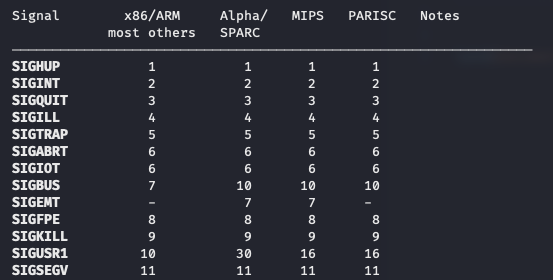
\includegraphics[height = 4cm]{asset/signals.png}
        \caption{Signals on Linux}
    \end{figure}

\end{frame}


\begin{frame}
    \frametitle{Using Signals}

    \begin{enumerate}
        \item Signal handler
        \item signal() syscall
    \end{enumerate}

\end{frame}